\begin{document}
\twocolumn[
\begin{center}
{\sffamily\bfseries\fontsize{14}{16}\selectfont
Mesclagem Laplaciana de Texturas em GPU:\\Avaliação de Salto de Níveis e Seleção Adaptativa sob Anisotropia\par}
\vspace{5pt}
{\fontsize{9.5}{11}\selectfont Ícaro Vinícius Carvalho Davi \quad Vinicius Macedo Colares Botelho \quad Caio Veloso Dias\par}
\vspace{2pt}
{\fontsize{8.5}{10}\selectfont Instituto Federal do Norte de Minas Gerais -- IFNMG, Campus Montes Claros\par
\texttt{\{ivcd, vmcb, cvd\}@aluno.ifnmg.edu.br}\par}
\end{center}
\begin{minipage}{0.94\textwidth}
\fontsize{8.5}{9.5}\selectfont
\noindent\textbf{Resumo.}
A composição de materiais por interpolação linear pode produzir costuras ou sobreposição de detalhes. Este trabalho avalia a mesclagem Laplaciana baseada em mipmaps, com ênfase no compromisso entre fidelidade à reconstrução de seis bandas e custo de execução. Reproduzimos a omissão de níveis descrita por Wronski e investigamos uma política contínua de seleção entre reconstrução completa, salto de níveis e mistura linear, orientada pela pegada projetada da textura. A avaliação reúne quatro casos bidimensionais, uma simulação em perspectiva e registros de um benchmark WebGL 2.0 em GPU AMD, com quatro câmeras, três configurações de material e duas resoluções de temporização. No albedo 2D, o subconjunto $\{0,\,2,\,4,\,6\}$ alcança 54,64 dB de PSNR, contra 32,87 dB do truncamento de mesmo orçamento. Nos quatro enquadramentos PBR a 1080p, esse salto reduz o tempo médio do passe entre 14,9\% e 25,3\%, mantendo PSNR de 50,09--54,33 dB em capturas independentes a $960\times540$. Na etapa histórica, a seleção adaptativa anisotrópica apresenta maior fidelidade que a isotrópica, mas perde competitividade relativa a 4K. Implementamos também um protocolo corrigido com resoluções coincidentes, consultas individuais e ablação controlada; 25 testes rápidos e três integrações WebGL foram aprovados em uma RTX 4050, incluindo validação real de 1080p/4K. Os resultados sustentam o salto par como alternativa consistente no conjunto avaliado e mostram que amostras lógicas, filtragem e tempo de GPU precisam ser analisados separadamente.
\par\vspace{3pt}
\noindent\textbf{Palavras-chave:} mesclagem de texturas; pirâmide Laplaciana; mipmapping; anisotropia; validação automatizada.
\par\vspace{5pt}
\noindent\textbf{Abstract.}
Linear material blending may introduce seams or overlapping details. We evaluate mipmap-based Laplacian blending, focusing on fidelity to a six-band reconstruction and execution cost. We reproduce Wronski's level-skipping approximation and investigate a continuous selection policy between full reconstruction, skipped levels, and linear blending, driven by the projected texture footprint. The evaluation combines four two-dimensional cases, a perspective simulation, and recorded WebGL 2.0 measurements on an AMD GPU, covering four camera presets, three material configurations, and two timing resolutions. For 2D albedo, the subset $\{0,\,2,\,4,\,6\}$ achieves 54.64 dB PSNR, compared with 32.87 dB for equal-budget truncation. Across four PBR views timed at 1080p, it reduces mean pass time by 14.9\%--25.3\%, with 50.09--54.33 dB PSNR from separate $960\times540$ captures. In the historical evaluation, anisotropic adaptive selection preserves more fidelity than isotropic selection, but becomes less competitive at 4K. We also implement a corrected protocol with matched resolutions, per-query records, and a controlled ablation; 25 fast tests and three WebGL integration tests pass on an RTX 4050, including actual 1080p/4K validation. These findings support even-level skipping within the tested dataset and show why logical samples, filtering, and GPU time require separate analysis.
\par\vspace{3pt}
\noindent\textbf{Keywords:} texture blending; Laplacian pyramid; mipmapping; anisotropy; GPU evaluation.
\end{minipage}\vspace{8pt}
]

\section{Introdução}
A composição de materiais permite representar mudanças de cobertura em terrenos, desgaste de superfícies e variações procedurais sem armazenar uma textura distinta para cada região. Duas imagens de material podem ser combinadas por uma máscara espacial que estabelece sua participação em cada ponto. O operador mais simples é uma combinação convexa por canal, implementada por \texttt{mix} em GLSL. Sua simplicidade favorece o uso em tempo real, mas uma única escala de transição não atende igualmente aos detalhes finos e às estruturas macroscópicas.

Uma transição curta pode revelar uma costura entre estruturas de baixa frequência, enquanto uma transição larga sobrepõe padrões independentes e reduz sua modulação. O problema aparece em albedo, mas também afeta a representação de relevo por mapas de normais. A aparência final depende, adicionalmente, da iluminação, da filtragem e da escala com que o material se projeta na imagem. Portanto, a avaliação de um operador de mesclagem deve distinguir a reconstrução do sinal de textura de sua aplicação em uma superfície iluminada.

As pirâmides multirresolução oferecem uma forma de atribuir transições diferentes às diferentes escalas do sinal \citep{burt1983laplacian,burt1983spline}. Na adaptação de \citet{wronski2025laplacian}, diferenças entre níveis de mipmaps substituem a construção explícita de uma pirâmide Laplaciana no shader. O uso de amostras adicionais motiva investigar aproximações que mantenham a aparência da reconstrução escolhida com menor custo.

Este estudo considera uma referência com seis bandas e residual no nível 6. Essa escolha fixa um alvo de comparação; não significa que seis bandas sejam sempre necessárias nem que a referência constitua a imagem fisicamente correta. A questão central é: \emph{como a seleção de níveis e a estimativa da pegada projetada alteram a fidelidade e o custo de uma implementação de mesclagem Laplaciana?} Desdobramos essa questão em duas hipóteses operacionais. Primeiro, alcançar o residual grosseiro com menos níveis pode aproximar melhor a referência que truncar a decomposição com o mesmo número de amostras. Segundo, a seleção adaptativa precisa considerar a anisotropia para evitar a simplificação prematura de detalhes visíveis.

As contribuições são uma avaliação reproduzível do salto de níveis já existente na literatura, uma caracterização algébrica de seu erro em relação à máscara multiescala e uma análise integrada dos caminhos completo, truncado, híbrido e adaptativo em albedo e materiais com normais. Acrescentamos um protocolo de avaliação com qualidade e tempo na mesma resolução, registro de consultas individuais e ablação controlada entre seleção e filtragem. Uma suíte automatizada verifica invariantes numéricos e exercita o caminho WebGL real, incluindo um controle negativo que detecta acoplamentos entre os fatores. A política adaptativa com reuso de amostras é estudada como decisão de implementação; não reivindicamos a invenção do salto de níveis nem da adaptação por minificação.

\section{Fundamentação e trabalhos relacionados}
\subsection{Mesclagem e estatísticas locais}
Sejam $X$ e $Y$ variáveis aleatórias que modelam valores de duas texturas, e $\alpha$ um peso fixo. A variância de sua mistura é
\begin{align}
\operatorname{Var}((1-\alpha)X+\alpha Y)
={}&(1-\alpha)^2\sigma_X^2+\alpha^2\sigma_Y^2\nonumber\\
&+2\alpha(1-\alpha)\operatorname{Cov}(X,Y).
\label{eq:variance}
\end{align}
Para fontes não correlacionadas com a mesma variância, a mistura no ponto médio retém metade dessa variância. Essa conclusão depende das hipóteses indicadas: não é um limite universal de perda para quaisquer imagens, nem uma previsão direta da variância local de uma máscara espacial variável. Fontes correlacionadas, frequências diferentes e a relação entre máscara e conteúdo modificam o resultado.

\citet{heitz2018high} tratam a preservação estatística na síntese por exemplo por meio de um operador com preservação de histograma. \citet{burley2019histogram} estuda uma formulação para tiling aleatório, enquanto \citet{mikkelsen2022practical} apresenta uma abordagem prática de hex-tiling. Essas linhas são relevantes porque a mesclagem deve preservar características da textura, e não simplesmente aumentar uma medida escalar de contraste. A fidelidade de um histograma também não caracteriza, isoladamente, a organização espacial dos padrões.

O operador Mix-Max de \citet{fournier2024mixmax} usa mapas de prioridade relacionados ao conteúdo para modelar a sobreposição de materiais e inclui tratamento de filtragem. Ele representa uma direção diferente da decomposição por bandas adotada aqui. O presente trabalho não implementa esses operadores como baselines; a comparação experimental restringe-se a variantes da família Laplaciana e à interpolação linear. Assim, os resultados não estabelecem superioridade sobre métodos de preservação de histograma ou sobre Mix-Max.

\subsection{Mesclagem multirresolução}
A pirâmide Laplaciana foi estudada como representação compacta de imagens \citep{burt1983laplacian}. A spline multirresolução aplica decomposição por escalas à composição de mosaicos \citep{burt1983spline}. Em vez de usar a mesma máscara para todos os detalhes, cada banda recebe um peso espacial compatível com sua escala. A reconstrução soma as bandas mescladas e um residual de baixa frequência. A ideia também aparece na fusão de exposições \citep{mertens2007exposure}.

A edição de imagens no domínio de gradientes \citep{perez2003poisson} oferece outra maneira de controlar descontinuidades. Contudo, resolver um problema global de composição e avaliar amostras locais dentro de um fragment shader são cenários computacionais diferentes. Nosso recorte favorece acesso local às cadeias de mipmaps já disponíveis e não exige um solucionador de equações de Poisson durante a renderização.

\subsection{Posicionamento em relação ao artigo-base}
\citet{wronski2025laplacian} descreve a avaliação direta de bandas a partir de mipmaps e, nas seções 6.1 e 6.2, discute minificação e salto de níveis. Essas operações pertencem ao trabalho-base. Aqui, a contribuição experimental consiste em confrontar escolhas concretas de níveis, estimadores isotrópico e anisotrópico e custos observados em uma implementação WebGL. A extensão não é apresentada como método inteiramente novo.

Essa distinção também evita interpretar o custo $3(K+1)$ como inerente a toda configuração do método. O fator três pressupõe duas texturas e uma máscara amostrada por nível. Materiais com mais canais, máscaras procedurais ou compartilhamento de leituras alteram a contagem. No experimento PBR, normais e rugosidade são empacotadas, produzindo um custo por nível distinto daquele do albedo isolado.

\section{Formulação da mesclagem}
\subsection{Notação e reconstrução completa}
Sejam $A_k(\mathbf{u})$ e $B_k(\mathbf{u})$ os níveis $k$ das texturas de entrada amostrados na mesma coordenada $\mathbf{u}$, após filtragem e interpolação espacial. Seja $M_k(\mathbf{u})$ o nível correspondente da máscara. Para simplificar a escrita, omitimos $\mathbf{u}$. Definimos
\begin{equation}
\mathcal{B}(a,b,m)=(1-m)a+mb.
\end{equation}
As bandas são diferenças entre níveis já amostrados na grade de reconstrução:
\begin{equation}
D^A_k=A_k-A_{k+1},\qquad D^B_k=B_k-B_{k+1}.
\end{equation}
A saída completa com $K$ bandas é
\begin{equation}
I_{\mathrm{full}}=\sum_{k=0}^{K-1}\mathcal{B}(D^A_k,D^B_k,M_k)
+\mathcal{B}(A_K,B_K,M_K).
\label{eq:full}
\end{equation}
O índice $K$ identifica o residual; portanto, $K=6$ requer sete níveis amostrados, de 0 a 6. Na configuração de albedo, são 21 amostras lógicas. A interpolação linear é o caso sem bandas, com apenas $\mathcal{B}(A_0,B_0,M_0)$.

A soma das diferenças de uma única fonte é telescópica:
\begin{equation}
\sum_{k=0}^{K-1}(A_k-A_{k+1})+A_K=A_0.
\end{equation}
Essa propriedade é algébrica e não exige que os filtros sejam Gaussianos ideais. Entretanto, a interpretação das bandas como faixas de frequência bem separadas depende dos filtros. Além disso, pesos distintos para cada banda impedem aplicar diretamente o cancelamento telescópico à mistura de duas fontes.

\subsection{Seleção de um subconjunto de níveis}
Considere uma sequência crescente $\mathcal{S}=(s_0,\ldots,s_q)$, com $s_0=0$. A saída genérica é
\begin{align}
I_{\mathcal S}={}&\sum_{j=0}^{q-1}\mathcal{B}(A_{s_j}-A_{s_{j+1}},
B_{s_j}-B_{s_{j+1}},M_{s_j})\nonumber\\
&+\mathcal{B}(A_{s_q},B_{s_q},M_{s_q}).
\label{eq:subset}
\end{align}
Cada banda agrupada usa a máscara de seu extremo mais fino. Avaliamos o conjunto completo $\{0,\,1,\,2,\,3,\,4,\,5,\,6\}$, truncamentos até 3, 4 e 5, o salto par $\{0,\,2,\,4,\,6\}$ e a variante híbrida $\{0,\,1,\,3,\,5\}$. Os dois últimos usam quatro níveis, mas apenas o salto par mantém o residual da referência. O híbrido conserva a primeira diferença fina e encerra a reconstrução em 5; a comparação envolve, portanto, simultaneamente agrupamento e mudança de residual.

\begin{table}[t]
\centering\small
\caption{Amostras lógicas por fragmento. A contagem inclui máscaras e depende dos mapas efetivamente amostrados.}
\label{tab:cost}
\begin{tabular}{lrrr}\toprule
Configuração & Albedo & PBR 2 & PBR 3\\\midrule
Linear, um nível & 3 & 5 & 8\\
Completa, sete níveis & 21 & 35 & 56\\
Truncada 3, quatro níveis & 12 & 20 & 32\\
Salto par, quatro níveis & 12 & 20 & 32\\
Híbrida, quatro níveis & 12 & 20 & 32\\\bottomrule
\end{tabular}
\end{table}

\subsection{O que a identidade telescópica preserva}
Se todos os níveis da máscara forem iguais a uma constante $m$, a Equação~\ref{eq:subset} se reduz a
\begin{equation}
I_{\mathcal S}=(1-m)A_0+mB_0.
\label{eq:constant}
\end{equation}
Logo, qualquer uma das sequências avaliadas reconstrói exatamente a mistura linear de máscara constante, a menos de arredondamento. Para $m=0$ ou $m=1$, recupera-se uma das fontes. Em uma máscara espacial, essa garantia só vale onde todos os níveis amostrados compartilham o mesmo peso. Estar fora da transição de $M_0$ não basta: níveis grosseiros podem incorporar regiões vizinhas da outra fonte.

Também é possível explicitar o erro introduzido ao agrupar duas bandas consecutivas. Para uma banda par iniciada em $k$, o agrupamento substitui $M_{k+1}$ por $M_k$ na segunda diferença. Definindo $\Delta_k=D^B_k-D^A_k$, obtemos, antes do recorte de faixa,
\begin{equation}
I_{\mathrm{par}}-I_{\mathrm{full}}
=\sum_{k\in\{0,2,4\}}(M_k-M_{k+1})\Delta_{k+1}.
\label{eq:error}
\end{equation}
O residual no nível 6 se cancela porque é comum às duas saídas. A Equação~\ref{eq:error} mostra por que preservar a soma das bandas de cada fonte não equivale a preservar a mistura ponderada. Há erro quando as máscaras diferem entre escalas e a banda omitida distingue as fontes.

Para cada canal, a desigualdade triangular fornece
\begin{equation}
|I_{\mathrm{par}}-I_{\mathrm{full}}|
\leq\sum_{k\in\{0,2,4\}}|M_k-M_{k+1}|\,|\Delta_{k+1}|.
\end{equation}
Esse limite organiza a interpretação, mas não garante erro pequeno para entradas arbitrárias. Máscaras detalhadas e fontes com forte diferença nas bandas agrupadas podem aumentar a discrepância. O recorte final para $[0,\,1]$ e a renormalização de normais introduzem operações não lineares posteriores, às quais a identidade de erro bruto não se aplica diretamente.

\section{Seleção adaptativa e implementação}
\subsection{Pegada projetada da textura}
Distância à câmera é apenas um indicador indireto da escala de textura: inclinação da superfície, resolução de saída e parametrização UV também importam. No caminho 3D, usamos derivadas de tela das coordenadas UV. Se $T$ é a resolução de referência da textura, definimos os vetores em unidades de texel
\begin{equation}
\mathbf{j}_x=T\,\partial\mathbf{u}/\partial x,\qquad
\mathbf{j}_y=T\,\partial\mathbf{u}/\partial y.
\end{equation}
As derivadas são calculadas antes das ramificações do shader. Para $a=\mathbf{j}_x\cdot\mathbf{j}_x$, $b=\mathbf{j}_y\cdot\mathbf{j}_y$ e $c=\mathbf{j}_x\cdot\mathbf{j}_y$, os comprimentos principais da pegada são
\begin{equation}
\rho_{\max,\min}=\sqrt{\frac{a+b\ \pm\sqrt{(a-b)^2+4c^2}}{2}},
\end{equation}
com limites positivos no código para evitar erros numéricos. O estimador isotrópico é $\lambda_{\mathrm{iso}}=\max(0,\log_2\rho_{\max})$. Para anisotropia máxima $a_{\max}=8$, usamos
\begin{equation}
\lambda_{\mathrm{aniso}}=\max\!\left(0,\log_2\max\left(\rho_{\min},\frac{\rho_{\max}}{a_{\max}}\right)\right).
\label{eq:aniso}
\end{equation}
O segundo estimador evita filtrar isotropicamente toda a pegada pela dimensão mais larga quando o hardware pode integrar ao longo de um eixo alongado.

No protocolo histórico (v1), o mesmo controle escolhia o estimador e alterava a amostragem: o caminho anisotrópico usava \texttt{textureGrad} em $k=0$ e \texttt{textureLod} em $\max(\lambda_{\mathrm{eff}},k)$ nos demais níveis; o isotrópico usava o segundo procedimento em todos eles. Essa comparação mistura seleção e filtragem. Seus resultados são preservados como avaliação de dois caminhos completos.

No protocolo corrigido (v2), separamos $\lambda_s$, usado para selecionar os regimes, de $\lambda_f$, usado na amostragem:
\begin{equation}
\lambda_s\in\{\lambda_{\mathrm{iso}},\lambda_{\mathrm{aniso}}\},\qquad
\lambda_f=\lambda_{\mathrm{aniso}}.
\label{eq:lodseparado}
\end{equation}
A filtragem inicial é outro fator independente: \texttt{textureGrad} com as derivadas originais, ou \texttt{textureLod} em $\lambda_f$. Para $k>0$, ambos usam \texttt{textureLod} em $\max(\lambda_f,k)$. Assim, mudar apenas $\lambda_s$ não altera ocultamente os níveis amostrados. A Seção~\ref{sec:v2} descreve a matriz de ablação e sua verificação em GPU.

\subsection{Política contínua e reuso}
Normalizamos o LOD de seleção como $\xi=\operatorname{clamp}(\lambda_s/4{,}5;\,0;\,1)$; em v1, $\lambda_s=\lambda_{\mathrm{eff}}$. No benchmark 3D, os centros de transição são $n=0{,}25$ e $f=0{,}65$, com meia largura $h=0{,}08$. Para $S(e_0,e_1,x)$ igual à função \texttt{smoothstep}, definimos
\begin{align}
u&=S(n-h,n+h,\xi),\quad v=S(f-h,f+h,\xi),\\
w_F&=(1-u)(1-v),\quad w_S=u(1-v),\quad w_L=v.
\end{align}
Os pesos são não negativos e somam um. A saída de cada propriedade, antes das operações finais de material, é
\begin{equation}
I_{\mathrm{adap}}=w_F I_{\mathrm{full}}+w_S I_{\mathrm{par}}+w_L I_{\mathrm{linear}}.
\label{eq:adaptive}
\end{equation}
Essa é a operação implementada no shader 3D: mistura das reconstruções, com compartilhamento das amostras necessárias. Não se trata apenas de alterar a máscara de uma única banda. A continuidade dos pesos evita um degrau deliberado na troca de regimes, mas não comprova ausência de cintilação temporal, aliasing ou popping em movimento.

Como $\{0\}\subset\{0,\,2,\,4,\,6\}\subset\{0,\ldots,6\}$, o conjunto de níveis necessário em uma faixa de transição é a união dos conjuntos dos regimes ativos. Uma transição completo--salto utiliza sete níveis; uma transição salto--linear utiliza quatro. Implementar os dois ramos de forma independente desperdiçaria leituras compartilhadas. O custo lógico é
\begin{equation}
C(\mathbf{p})=c_m\left|\bigcup_{r:w_r(\mathbf{p})>0}\mathcal{S}_r\right|,
\label{eq:union}
\end{equation}
onde $c_m$ é 3, 5 ou 8 conforme o material da Tabela~\ref{tab:cost}. O contador no shader registra essa quantidade, não transações físicas de memória nem ocupação medida das unidades de textura.

\begin{lstlisting}[language=C,caption={Pseudocódigo do reuso no caminho adaptativo. Reconstruções compartilham leituras do mesmo nível.},label={lst:reuse}]
w = regimeWeights(projectedFootprint);
levels = unionOfActiveLevelSets(w);
for (int k : levels) {
    cache[k] = sampleMaterialAndMasks(k);
}
full = w.full > 0 ? reconstruct(cache, FULL) : 0;
skip = w.skip > 0 ? reconstruct(cache, EVEN) : 0;
lin  = w.lin  > 0 ? residual(cache[0]) : 0;
result = w.full*full + w.skip*skip + w.lin*lin;
\end{lstlisting}

\subsection{Representação dos materiais}
A implementação usa Python/NumPy/Pillow/SciPy para o caminho offline e WebGL 2.0/GLSL ES 3.00 com Three.js 0.149.0 para o caminho de GPU. O terreno tem $400\times400$ unidades, uma grade de $256\times256$ segmentos e repetição de textura equivalente a blocos de 10 unidades. A altura combina funções senoidais determinísticas, e as normais geométricas são obtidas de suas derivadas analíticas. As quatro câmeras fixam enquadramentos panorâmico, rasante, próximo e aéreo, todos com campo de visão de $50^\circ$.

No modo albedo, cada nível requer duas cores e uma máscara. Em PBR de duas camadas, cada textura de normais armazena rugosidade no canal alfa, elevando a contagem a cinco amostras por nível. A rugosidade é uma função determinística da luma do albedo, não uma medição independente do material. O modo de três camadas acrescenta cor, normal/rugosidade e segunda máscara, totalizando oito amostras por nível. A terceira camada é derivada de ativos existentes; ela avalia complexidade do pipeline, não diversidade independente de dados.

A composição de três camadas é hierárquica: primeiro mistura as duas fontes iniciais e depois a terceira. O peso desta última inclui um fator relacionado à altura do terreno. Após a reconstrução, o albedo é limitado a $[0,\,1]$; a normal codificada é decodificada, seu componente $z$ recebe limite inferior de 0,08 e o vetor é normalizado. A rugosidade é limitada a $[0{,}08;\,1]$. A iluminação emprega um modelo microfacetado GGX/Cook--Torrance, termo ambiente e neblina. Essas operações são compartilhadas pelas variantes de uma mesma configuração, mas tornam a comparação de quadros diferente da comparação de texturas sem iluminação.

\section{Metodologia experimental}
\subsection{Proveniência e rastreabilidade}
A fonte dos experimentos históricos é a revisão \texttt{10293a4} da branch \texttt{checkpoint-2-trabalho}. Os dados 2D, 3D e de GPU estão, respectivamente, nos arquivos \texttt{resultados\_checkpoint2.json}, \texttt{resultados\_3d.json} e \texttt{resultados\_gpu.json} de v1. A implementação v2 está na branch \texttt{benchmark-validacao}; seus registros têm \texttt{schemaVersion=2} e são apresentados separadamente. Os dados preservados, as tabelas geradas e o manifesto SHA-256 permitem distinguir as duas etapas, sem converter ou misturar medições antigas com novas.

Na consolidação, reexecutamos os quatro casos numéricos 2D com uma repetição por variante para verificar as métricas determinísticas e recalculamos SSIM dos quadros de GPU preservados. As durações de CPU dessa verificação não substituem as medições anteriores. Os tempos de desempenho históricos são os registros de 21 de novembro de 2026, cujo dataset preserva agregados, mas não consultas individuais nem sua contagem válida. As consultas de validação de v2 foram coletadas em 24 de novembro de 2026, em outro equipamento, com dados individuais preservados; elas não substituem ou reconstituem as sessões históricas.

As imagens de albedo e suas rotações acompanham a demonstração suplementar, com atribuição a Deliot e Heitz em \emph{GPU Zen 2}; os mapas de normais são atribuídos a ambientCG sob CC0 no arquivo de créditos. A avaliação usa esse conjunto disponibilizado, sem afirmar que imagens rotacionadas constituam amostras estatisticamente independentes. A nomenclatura ``Perlin'' identifica o arquivo de máscara fornecido; não assumimos acesso ao gerador ou à semente que o originou.

\subsection{Três camadas de avaliação}
\textbf{Bancada 2D.} São quatro casos: albedo original com máscara orgânica, duas texturas rotacionadas com a mesma máscara e um par de normais com máscara em rampa ou orgânica. O albedo tem $1024\times1024$ pixels e as normais, $512\times512$. A máscara orgânica é
\begin{equation}
M_0=\operatorname{clamp}(8(P-0{,}55)+0{,}5,0,1).
\end{equation}
Os níveis são reduzidos diretamente da entrada em modo \texttt{F} do Pillow, por canal, e ampliados bilinearmente para a grade original. O caminho principal usa BOX e \texttt{float32}, sem quantização intermediária para oito bits. BOX direto e BOX em cascata são equivalentes para essa grade de potência de dois, a menos de arredondamento. Essa equivalência não é assumida para outros filtros. O estudo de filtros aplica as opções BOX, BILINEAR, BICUBIC e LANCZOS do Pillow ao caso de albedo original. Não identificamos a opção LANCZOS do Pillow como Lanczos de suporte dois.

\textbf{Simulação 3D.} O script Python calcula interseções de raios com o campo de altura, derivadas analíticas e amostragem de pirâmides BOX em cascata. Avalia quatro câmeras no albedo, duas no PBR de duas camadas e a panorâmica no PBR de três camadas, a $960\times540$. Trata-se de simulação em CPU, com aproximação da filtragem anisotrópica; seus tempos não são tempos de GPU. A interseção com superfície analítica e a malha triangular do WebGL também não são implementações idênticas. A comparação entre elas é de tendência, sem exigir igualdade pixel a pixel.

\textbf{Renderização WebGL histórica.} O registro de hardware identifica \texttt{AMD Radeon Graphics (radeonsi renoir ACO)}, via ANGLE/OpenGL ES 3.2, Chromium headless 152 em Linux. Há suporte à extensão de consultas de tempo de GPU e anisotropia máxima de 16, limitada a 8 no teste. São oito configurações de cena/resolução/material e sete métodos, totalizando 56 registros agregados: quatro câmeras PBR 2 a 1080p; panorâmica com albedo e PBR 3 a 1080p; panorâmica e rasante PBR 2 a 4K.

\subsection{Regiões e métricas}
Para uma imagem candidata $I$ e uma referência $R$, ambas com faixa nominal unitária, calculamos
\begin{equation}
\mathrm{PSNR}=10\log_{10}\frac{1}{\mathrm{MSE}},\qquad
\mathrm{MSE}=\frac{1}{3|\Omega|}\sum_{\mathbf p\in\Omega}\|I(\mathbf p)-R(\mathbf p)\|_2^2.
\label{eq:psnr}
\end{equation}
PSNR infinito na referência indica autoidentidade, não qualidade perceptiva absoluta. SSIM \citep{wang2004ssim} é calculado sobre luma, com pesos $(0{,}2989;\,0{,}5870;\,0{,}1140)$, janela Gaussiana de desvio 1,5, suporte $11\times11$ e constantes $0{,}01^2$ e $0{,}03^2$.

Na bancada 2D, PSNR e SSIM são globais. Apenas a variância local média usa centros com $0{,}05<M_0<0{,}95$; sua janela é $7\times7$. Essa região contém 209.854 pixels no albedo orgânico, 52.386 nas normais orgânicas e 235.520 na rampa de normais. A taxa de overshoot considera a imagem inteira antes do recorte e conta pixels com pelo menos um canal fora de $[0,\,1]$. O erro angular compara vetores decodificados e normalizados em toda a imagem. Ele mede desvio da referência, não a correção física da normal resultante.

No 3D, PSNR considera pixels que atingem o terreno; o céu é excluído. Para SSIM dos quadros históricos preservados, o código erode a máscara de terreno com uma estrutura $9\times9$. Como o suporte de SSIM é $11\times11$, essa erosão não elimina necessariamente toda a influência da borda em todos os centros. Mantemos o procedimento para reproduzir os números, registrando a limitação em vez de afirmar isolamento estrito das janelas.

Há três resoluções diferentes no benchmark de GPU: a temporização usa $1920\times1080$ ou $3840\times2160$; PSNR é obtido em renderização separada a $960\times540$; SSIM é calculado dos PNGs a $1280\times720$. Os valores de PSNR e SSIM reutilizados nas linhas de 1080p e 4K não são medições de qualidade nessas resoluções de temporização. Para os métodos adaptativos, cuja seleção depende das derivadas, essa distinção é particularmente relevante.

\subsection{Temporização e contagem de amostras}
No protocolo histórico, o runner usa alvos offscreen RGBA de oito bits com profundidade e \texttt{pixelRatio=1}. Prepara as máscaras antes da medição e desativa avatar e visualizações de depuração. Cada configuração recebe 12 renderizações iniciais da referência, distribuídas em quatro ticks; seguem três rodadas de aquecimento e 25 rodadas de coleta. A ordem dos métodos alterna entre direta e reversa em cada rodada. A janela de consulta envolve \texttt{renderer.render}, incluindo o terreno e o céu. Portanto, medimos o passe de cena, e não apenas instruções isoladas do operador.

O tempo é obtido por \texttt{EXT\_disjoint\_timer\_query\_webgl2}. Consultas disponíveis são aceitas se o sinal de disjunção não estiver ativo no momento de leitura; consultas pendentes são descartadas após o prazo do runner. Leituras de framebuffer ficam fora da região temporizada. O caminho alternativo de cronômetro de CPU existe no código, mas todos os 56 registros analisados indicam consulta de GPU. Reportamos média, desvio padrão descritivo e, quando pertinente, mediana. Não calculamos intervalos de confiança sem os dados por rodada.

A redução relativa de tempo é $100(1-t/t_{\mathrm{ref}})$. Embora o JSON use o nome \texttt{speedup\_vs\_ref\_pct}, essa expressão mede redução percentual de duração, não aumento percentual de throughput. Uma redução de 23,8\% corresponde a uma razão de tempos de aproximadamente $1{,}31\times$, e não $1{,}238\times$.

O custo lógico é extraído em um passe de telemetria a $320\times180$, que codifica contador de amostras, regime e LOD. Um fator de escala das derivadas aproxima a resolução temporizada. A média se refere aos pixels do terreno nessa grade, não ao framebuffer completo; pequenos erros de quantização e diferenças de cobertura são possíveis. Filtragem bilinear, trilinear e anisotrópica podem envolver múltiplos texels para cada instrução lógica. Assim, a telemetria não mede banda de memória nem saturação de TMUs.

\section{Resultados do protocolo histórico}
\subsection{Albedo 2D e normais}
A Tabela~\ref{tab:2d} reúne os resultados do caso orgânico de albedo e das normais orgânicas. Com o mesmo orçamento de 12 amostras, o salto par apresenta 54,64 dB de PSNR no albedo, contra 32,87 dB do truncamento até 3. A diferença de 21,77 dB mostra que manter o residual grosseiro pode ser mais relevante que visitar apenas níveis consecutivos. O híbrido alcança 37,62 dB e se aproxima do truncamento até 5, coerentemente com seu residual no nível 5.

\begin{table}[t]
\centering\scriptsize\setlength{\tabcolsep}{3.2pt}
\caption{Bancada 2D: métricas globais contra a referência completa. Albedo: par original e máscara orgânica. Normais: mesmo tipo de máscara, em resolução própria. SSIM arredondado não significa identidade.}
\label{tab:2d}
\begin{tabular}{lrrrr}\toprule
Método & Amostras & PSNR albedo & SSIM & Ângulo normal\\
 & & (dB) & & (graus)\\\midrule
Linear & 3 & 32,21 & 0,9957 & 1,105\\
Truncado 3 & 12 & 32,87 & 0,9967 & 0,801\\
Truncado 4 & 15 & 34,19 & 0,9977 & 0,548\\
Truncado 5 & 18 & 37,65 & 0,9990 & 0,296\\
Completo 6 & 21 & $\infty$ & 1,0000 & 0,000\\
Salto par & 12 & 54,64 & 1,0000 & 0,331\\
Híbrido & 12 & 37,62 & 0,9990 & 0,466\\
Adaptativo 2D & 13,98$^*$ & 38,69 & 0,9989 & 0,436\\\bottomrule
\end{tabular}
\par\vspace{2pt}\raggedright\scriptsize $^*$Modelo com união de amostras; não é medição de execução da seleção espacial em GPU. A média nas normais é 13,97.
\end{table}

No par rotacionado, o salto par obtém 55,34 dB, enquanto o truncado 3 obtém 32,92 dB. Isso confirma a tendência sob rotação, mas não amplia a avaliação a uma nova família de materiais. Para normais com máscara orgânica, o erro angular do salto par é $0{,}331^\circ$, inferior a $0{,}801^\circ$ do truncamento 3 e superior a $0{,}296^\circ$ do truncamento 5. Portanto, o salto não domina todas as alternativas em todas as métricas; sua vantagem mais clara é o compromisso de qualidade sob orçamento equivalente.

A rampa de normais torna a comparação muito menos discriminante: a mistura linear já atinge 69,54 dB, contra 81,29 dB do salto par, e o erro angular cai de $0{,}018^\circ$ para $0{,}003^\circ$. Uma máscara suave em escala ampla altera pouco os pesos entre níveis; esse comportamento é compatível com a Equação~\ref{eq:error}. Ele também mostra que médias globais podem esconder diferenças localizadas na faixa de transição.

A variância local do albedo orgânico é 0,009528 no linear, 0,009357 na referência e 0,009376 no salto par. Como o linear tem valor maior, seria incorreto apresentar esse caso como aumento medido de variância causado pela mesclagem Laplaciana. A distribuição espacial de detalhes e a coerência da transição são relevantes, e variância elevada também pode resultar de artefatos. Usamos a métrica como descrição complementar, sem convertê-la automaticamente em qualidade perceptiva.

\subsection{Sensibilidade ao filtro e overshoot}
A Tabela~\ref{tab:filters} apresenta o estudo de filtros com reconstrução completa no albedo original. Todas as comparações de PSNR e SSIM usam BOX como referência e, portanto, medem mudança de operador de filtragem, não a aproximação do salto de níveis.
\begin{table}[t]
\centering\small
\caption{Filtros do Pillow na bancada 2D. Overshoot é medido antes do recorte final, sobre todos os pixels.}
\label{tab:filters}
\begin{tabular}{lrrr}\toprule
Filtro & PSNR vs. BOX (dB) & SSIM & Overshoot (\%)\\\midrule
BOX & $\infty$ & 1,0000 & 0,633\\
BILINEAR & 48,24 & 0,9999 & 0,639\\
BICUBIC & 51,45 & 1,0000 & 0,910\\
LANCZOS & 47,84 & 0,9999 & 0,835\\\bottomrule
\end{tabular}
\end{table}
BOX produz valores brutos entre $-0{,}0788$ e $1{,}1019$; filtros de maior suporte também extrapolam a faixa. O recorte é, portanto, uma operação efetiva, e não apenas preventiva. BICUBIC apresenta a maior proporção de pixels extrapolados neste caso. O conjunto não permite afirmar que um filtro seja perceptivamente superior em geral nem que os quatro sejam equivalentes.

Nas normais orgânicas, a taxa de overshoot bruto é 5,713\% na referência e 6,146\% no salto par; o híbrido reduz esse valor a 4,369\%, mas aumenta o desvio angular para $0{,}466^\circ$. A renormalização produz vetores unitários após a mistura, porém não restaura a distribuição de orientações perdida nem converte o erro angular em avaliação de aparência especular. Esse compromisso reforça a necessidade de observar o material iluminado.

\subsection{Simulação em perspectiva}
A Tabela~\ref{tab:cpu3d} resume o albedo na simulação 3D. O salto par mantém PSNR de 55,05--59,87 dB nas quatro câmeras. A variante adaptativa anisotrópica apresenta PSNR superior ao caminho isotrópico em todas elas, com diferença especialmente expressiva no ângulo rasante: 47,16 contra 29,64 dB.
\begin{table}[t]
\centering\scriptsize\setlength{\tabcolsep}{4pt}
\caption{Simulação 3D em CPU a $960\times540$, albedo. PSNR no terreno. A última coluna é custo lógico médio do adaptativo anisotrópico; a referência usa 21 amostras.}
\label{tab:cpu3d}
\begin{tabular}{lrrrr}\toprule
Câmera & Salto par & Adap. iso. & Adap. aniso. & Amostras\\
 & \multicolumn{3}{c}{PSNR (dB)} & aniso.\\\midrule
Panorâmica & 58,21 & 33,87 & 41,56 & 8,29\\
Rasante & 55,05 & 29,64 & 47,16 & 17,58\\
Próxima & 57,90 & 31,10 & 45,96 & 16,34\\
Aérea & 59,87 & 37,02 & 38,30 & 3,45\\\bottomrule
\end{tabular}
\end{table}

O custo adaptativo depende da cobertura dos regimes. Na câmera aérea, a maior parte do terreno usa mistura linear, aproximando-se de três amostras; na câmera rasante, detalhes continuam resolvíveis em uma direção e a política anisotrópica mantém mais reconstrução multiescala. O baixo custo isotrópico resulta, em parte, de descartar conteúdo que a referência anisotrópica preserva. Não deve ser interpretado como ganho de eficiência a qualidade constante.

No PBR 2, o PSNR do salto par é 54,11 dB na panorâmica e 51,61 dB na rasante. A variante adaptativa anisotrópica alcança, respectivamente, 38,81 e 44,31 dB. A proximidade dessas tendências com os quadros WebGL fornece uma verificação qualitativa entre implementações. Diferenças de filtragem, geometria e quantização impedem tratar os valores da simulação como substitutos exatos dos resultados de GPU.

\subsection{Tempos registrados em GPU}
A Tabela~\ref{tab:gpu} apresenta as quatro configurações PBR 2 com duas resoluções. No enquadramento panorâmico a 1080p, o salto par reduz a média de 11,389 para 8,673 ms, ou 23,8\%. O truncamento de mesmo orçamento leva 9,519 ms. Como o sombreamento, o céu e o rasterizador também participam da consulta, a redução de 42,9\% nas amostras lógicas não se converte na mesma redução de duração.

\begin{table*}[t]
\centering\small\setlength{\tabcolsep}{5pt}
\caption{Tempos históricos do passe de cena na GPU AMD, em ms (média $\pm$ desvio padrão descritivo). O PSNR é de uma captura separada a $960\times540$, não de 1080p ou 4K. Cada configuração prevê 25 rodadas de coleta; consultas individuais não estão preservadas.}
\label{tab:gpu}
\begin{tabular}{lrrrrrr}\toprule
 & \multicolumn{2}{c}{Panorâmica} & \multicolumn{2}{c}{Rasante} & \multicolumn{2}{c}{PSNR (dB)}\\
Método & 1080p & 4K & 1080p & 4K & Panorâmica & Rasante\\\midrule
Linear & $6{,}509\pm0{,}117$ & $12{,}784\pm0{,}807$ & $5{,}053\pm0{,}921$ & $9{,}260\pm0{,}275$ & 33,52 & 31,47\\
Completo 6 & $11{,}389\pm0{,}079$ & $19{,}266\pm0{,}893$ & $8{,}877\pm1{,}709$ & $15{,}383\pm0{,}292$ & $\infty$ & $\infty$\\
Truncado 3 & $9{,}519\pm0{,}098$ & $17{,}047\pm0{,}369$ & $7{,}417\pm1{,}326$ & $13{,}754\pm0{,}235$ & 32,91 & 31,89\\
Salto par & $8{,}673\pm0{,}086$ & $15{,}814\pm0{,}557$ & $7{,}023\pm1{,}319$ & $13{,}153\pm0{,}341$ & 52,67 & 50,09\\
Híbrido & $9{,}090\pm0{,}104$ & $16{,}269\pm0{,}345$ & $7{,}178\pm1{,}347$ & $13{,}455\pm0{,}280$ & 37,10 & 36,87\\
Adaptativo iso. & $3{,}587\pm0{,}102$ & $5{,}982\pm0{,}213$ & $4{,}068\pm0{,}804$ & $7{,}619\pm0{,}154$ & 27,69 & 25,91\\
Adaptativo aniso. & $9{,}015\pm0{,}127$ & $18{,}017\pm0{,}293$ & $7{,}763\pm1{,}413$ & $14{,}715\pm0{,}280$ & 38,72 & 44,05\\\bottomrule
\end{tabular}
\end{table*}

\begin{figure*}[t]
\centering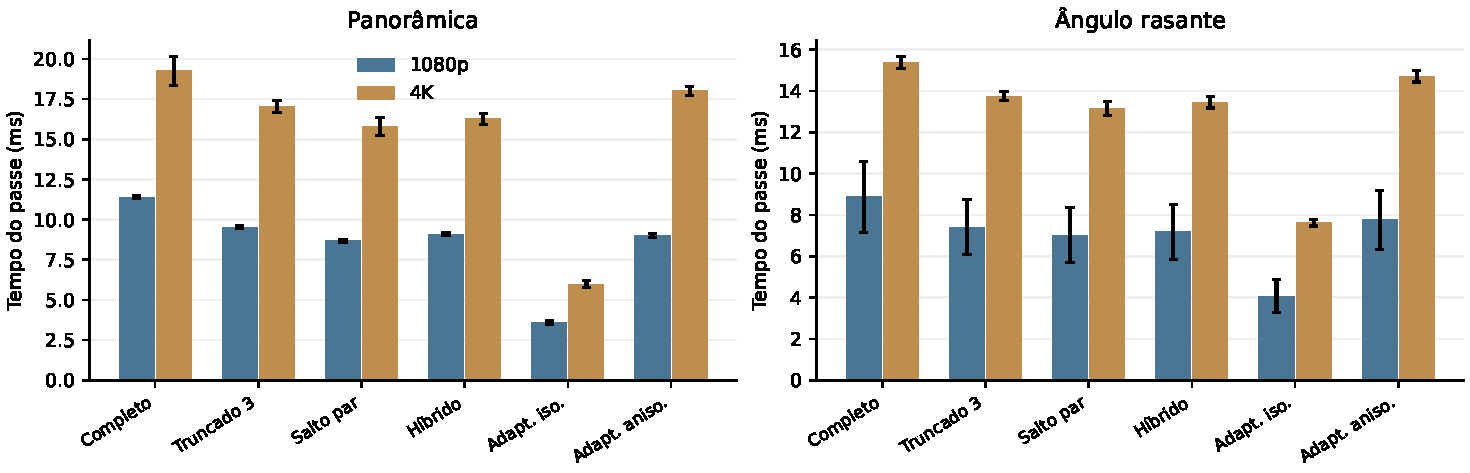
\includegraphics[width=0.97\textwidth]{figures/tempos.pdf}
\caption{Temporização do passe de cena, com barras de desvio padrão. As duas resoluções usam o mesmo material PBR 2 e câmeras fixas. A redução de duração difere da redução do contador lógico de amostras.}
\label{fig:time}
\end{figure*}

A Figura~\ref{fig:time} evidencia a mudança de comportamento a 4K. Na panorâmica, o salto par reduz o tempo de 19,266 para 15,814 ms, uma redução de 17,9\%; o adaptativo anisotrópico atinge 18,017 ms, apenas 6,5\% abaixo da referência. Na rasante a 4K, o salto par reduz 14,5\% e o adaptativo anisotrópico, 4,3\%. A política adaptativa pode exigir mais níveis quando o aumento de resolução torna os detalhes visíveis. Custos de seleção e execução dos ramos também participam do tempo observado, mas os agregados não permitem atribuir causalmente a diferença a um único componente microarquitetural.

As câmeras próxima e aérea, medidas somente a 1080p em PBR 2, produzem médias de 6,576 e 4,344 ms para a referência; o salto par reduz esses valores a 5,595 e 3,244 ms. Assim, a redução do salto nos quatro enquadramentos é 14,9--25,3\%. O adaptativo anisotrópico reduz 8,6\% na câmera próxima e 32,9\% na aérea, mostrando dependência mais forte do enquadramento.

Os dados rasantes a 1080p têm dispersão elevada: a referência apresenta média de 8,877 ms e mediana de 9,904 ms, com desvio de 1,709 ms. O salto par apresenta média de 7,023 e mediana de 7,791 ms. Usando medianas, a redução correspondente é aproximadamente 21,3\%, próxima dos 20,9\% calculados com médias. A tendência é semelhante, mas a distribuição não pode ser reconstruída apenas de seus resumos; não inferimos estabilidade temporal ou significância estatística a partir deles.

\subsection{Complexidade de material e qualidade dos quadros}
\begin{table}[t]
\centering\small\setlength{\tabcolsep}{4pt}
\caption{Panorâmica a 1080p: escalabilidade do passe conforme o material. Tempos em ms; amostras correspondem ao completo/salto.}
\label{tab:material}
\begin{tabular}{lrrrr}\toprule
Material & Amostras & Completo & Salto & Adap. aniso.\\\midrule
Albedo & 21/12 & 2,570 & 2,107 & 2,105\\
PBR 2 & 35/20 & 11,389 & 8,673 & 9,015\\
PBR 3 & 56/32 & 11,634 & 8,234 & 8,535\\\bottomrule
\end{tabular}
\end{table}
A Tabela~\ref{tab:material} mostra que mais amostras não implicam crescimento monotônico do tempo entre sessões/configurações. PBR 3 usa mais mapas, mas seu salto é ligeiramente mais rápido que o de PBR 2 nos registros. Conteúdo, caminhos compilados e condições de execução podem contribuir. Sem amostras brutas, controle adicional de clocks e repetição de sessões, não atribuímos o fenômeno a melhor escalabilidade de três materiais. A comparação mais controlada é entre variantes da mesma configuração.

\begin{figure*}[t]
\centering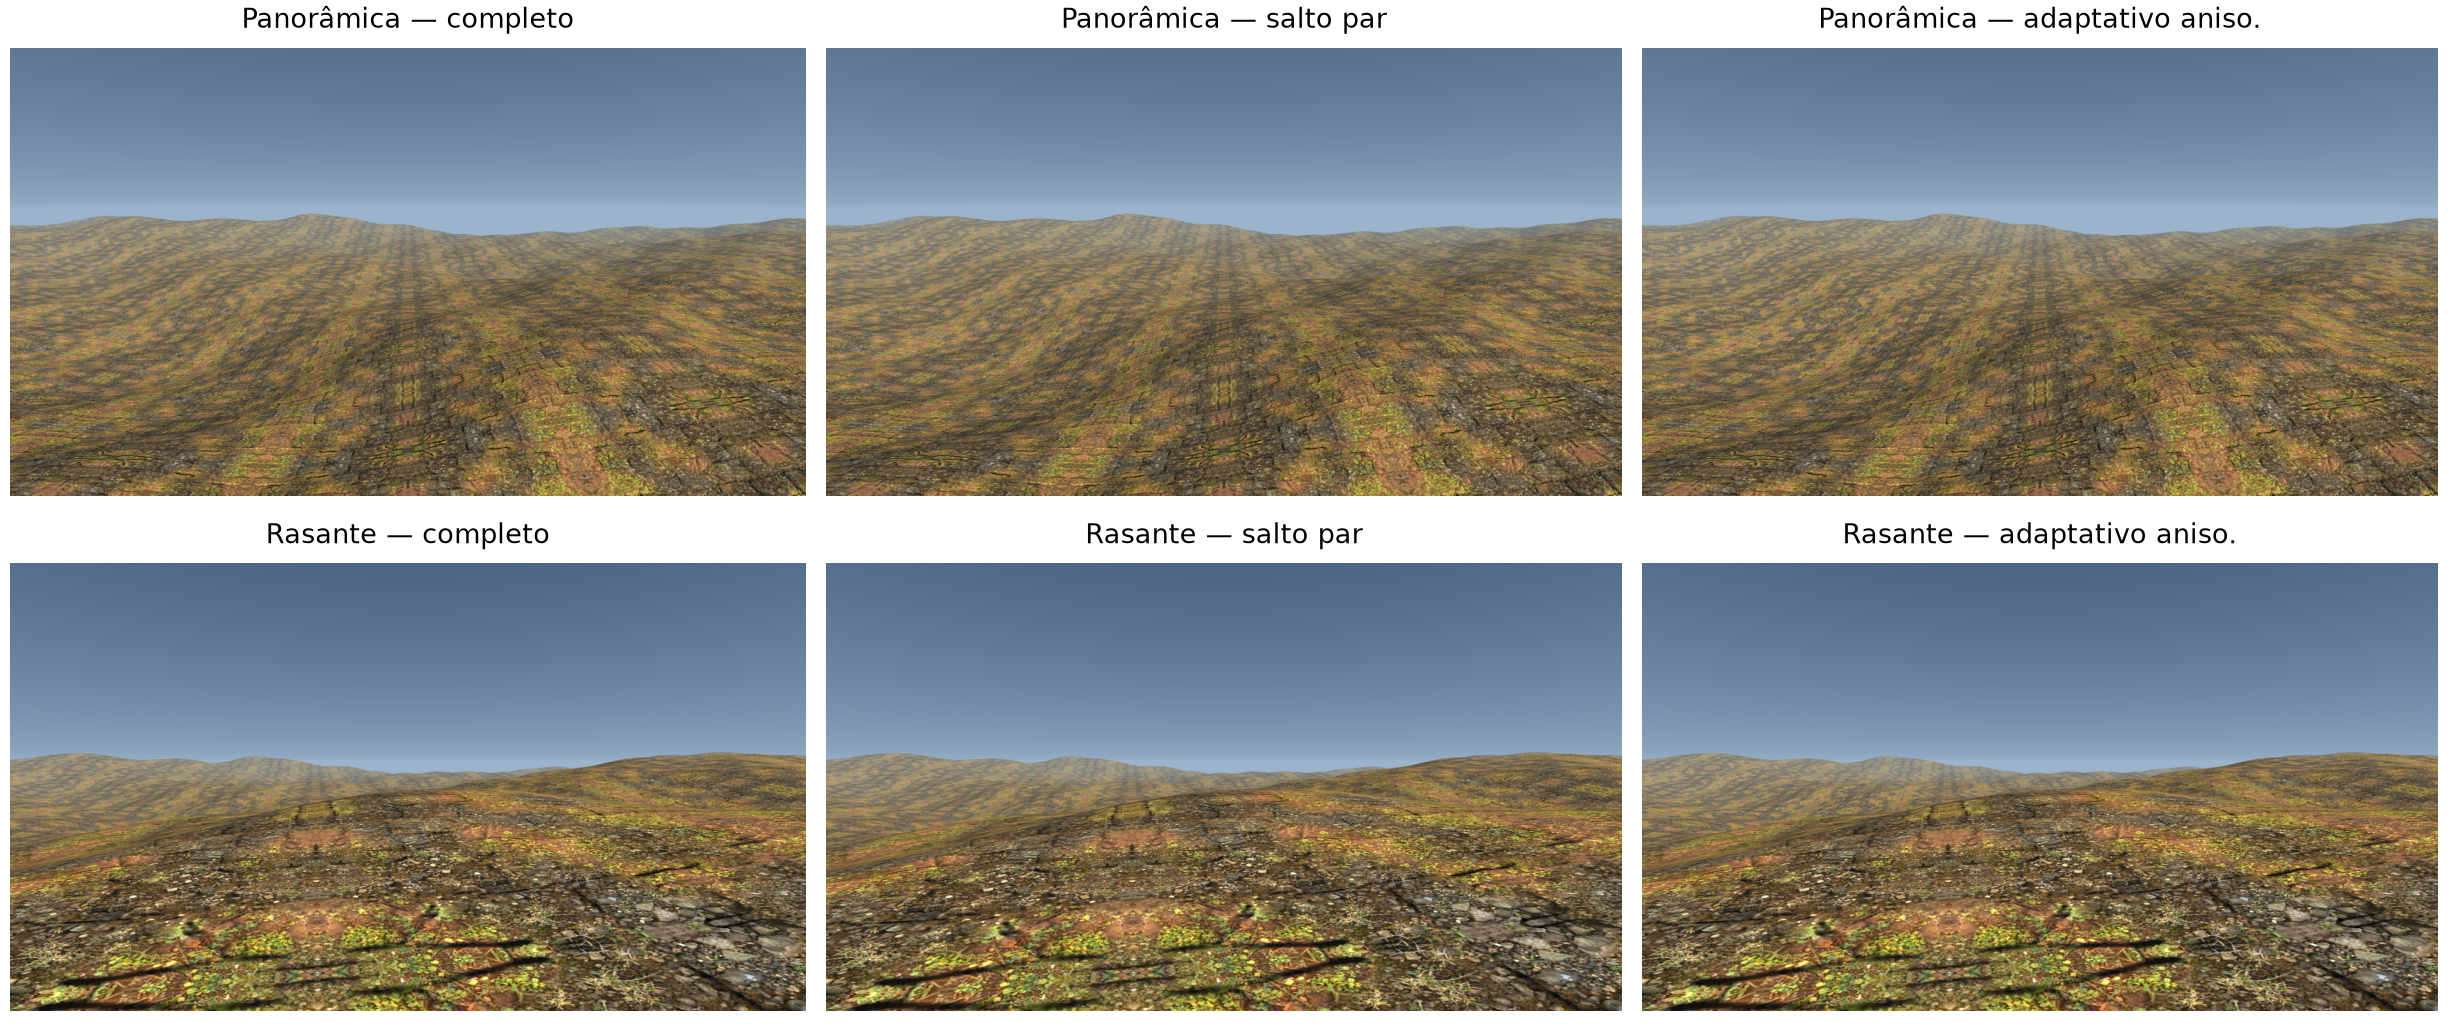
\includegraphics[width=0.98\textwidth]{figures/painel_gpu.png}
\caption{Quadros WebGL preservados a $1280\times720$, PBR 2. Colunas: completo, salto par e adaptativo anisotrópico; linhas: panorâmica e rasante. As imagens ilustram aparência nessa resolução de captura, independentemente da resolução usada para medir tempo.}
\label{fig:frames}
\end{figure*}

Na panorâmica PBR 2, o salto par tem SSIM de 0,9993 nos quadros preservados; na rasante, 0,9996. O adaptativo anisotrópico apresenta 0,9829 e 0,9945, enquanto o isotrópico cai a 0,7078 e 0,7976. A Figura~\ref{fig:frames} permite inspecionar a aparência em conjunto, mas diferenças pequenas exigem recortes e métricas. Não realizamos estudo com observadores para estabelecer limiar de imperceptibilidade.

\begin{figure*}[t]
\centering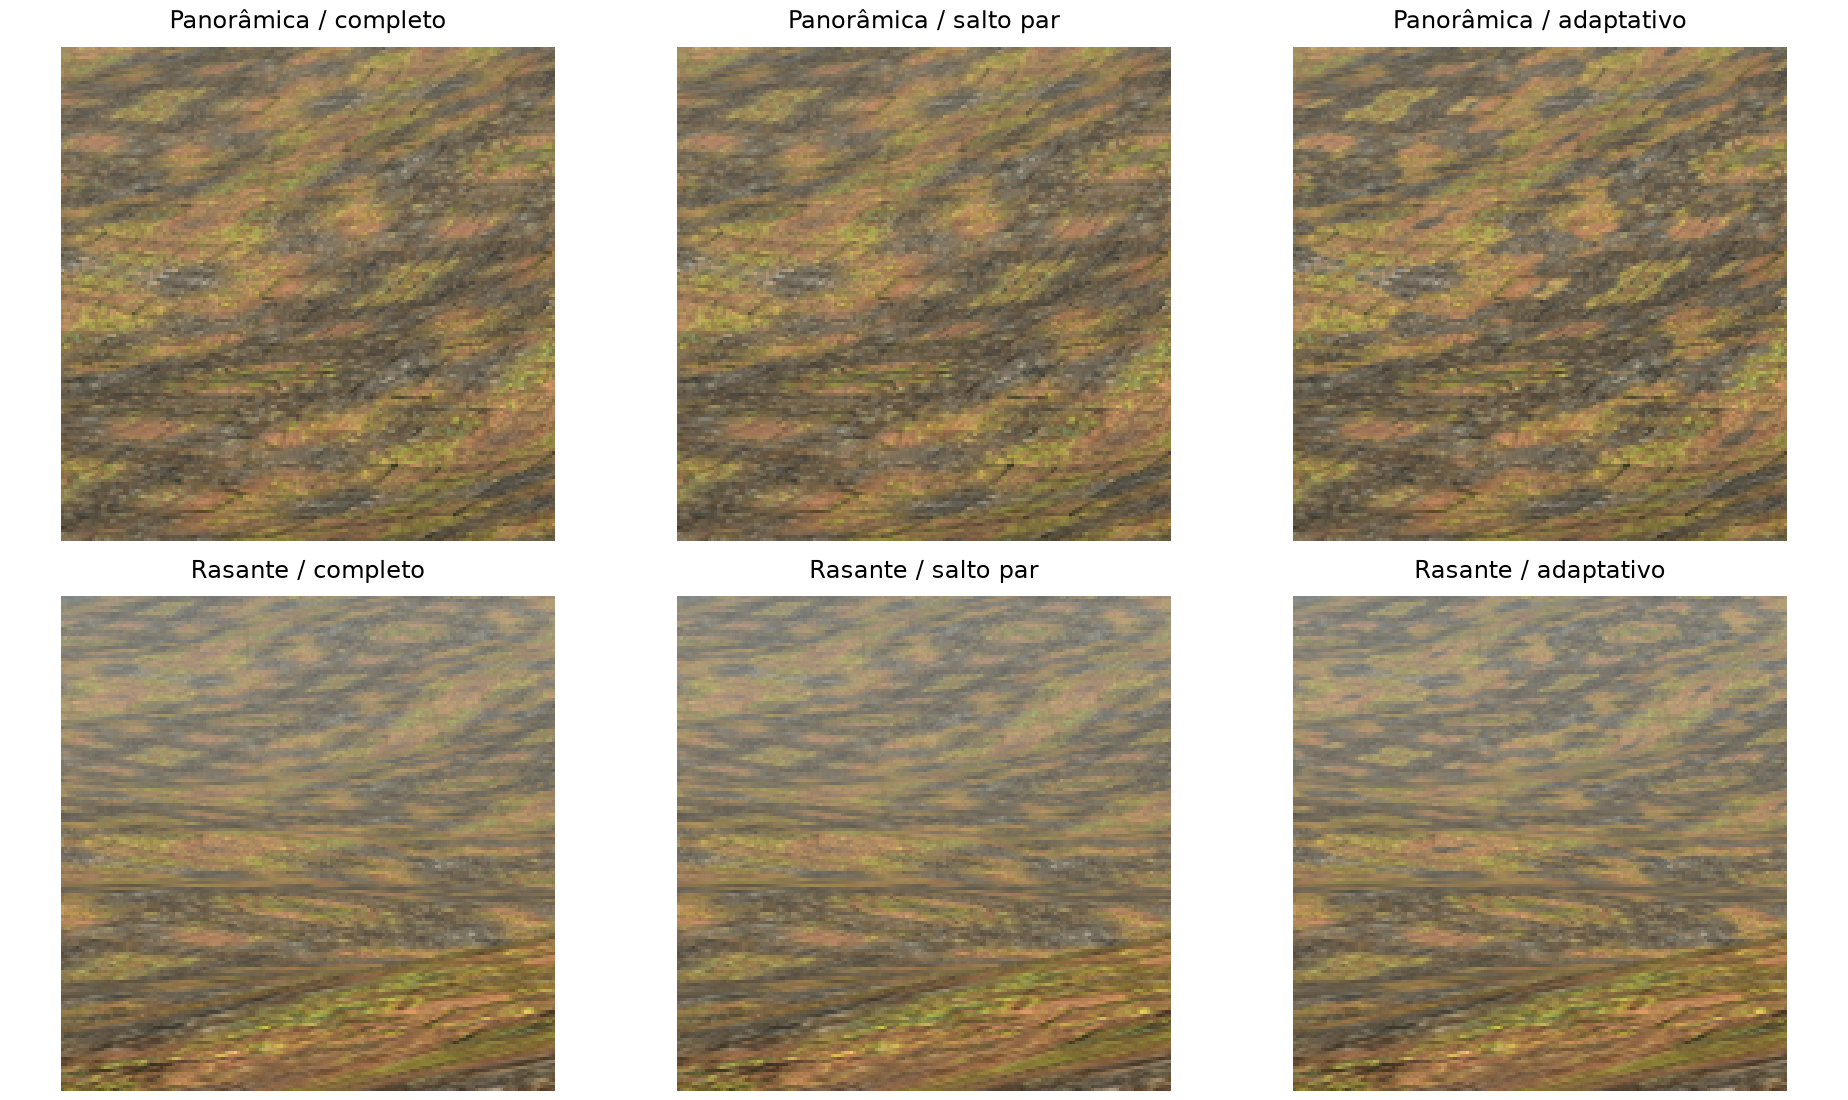
\includegraphics[width=0.88\textwidth]{figures/recortes.png}
\caption{Recortes $160\times160$ sem interpolação, extraídos dos quadros $1280\times720$. Para cada câmera, o centro é escolhido no maior erro RGB médio do adaptativo anisotrópico dentro do terreno e ajustado para manter o recorte na imagem. É uma seleção dirigida a falhas, não uma amostra aleatória. As coordenadas estão no registro de verificação.}
\label{fig:crops}
\end{figure*}

A Figura~\ref{fig:crops} concentra a inspeção onde a discrepância adaptativa é maior. O salto par conserva o residual de baixa frequência da referência e apresenta diferença global pequena; a seleção adaptativa substitui parte da reconstrução por mistura linear e pode alterar regiões maiores. Esse comportamento é consistente com seus PSNRs menores, ainda que a economia de tempo seja favorável em algumas câmeras.

\begin{figure*}[t]
\centering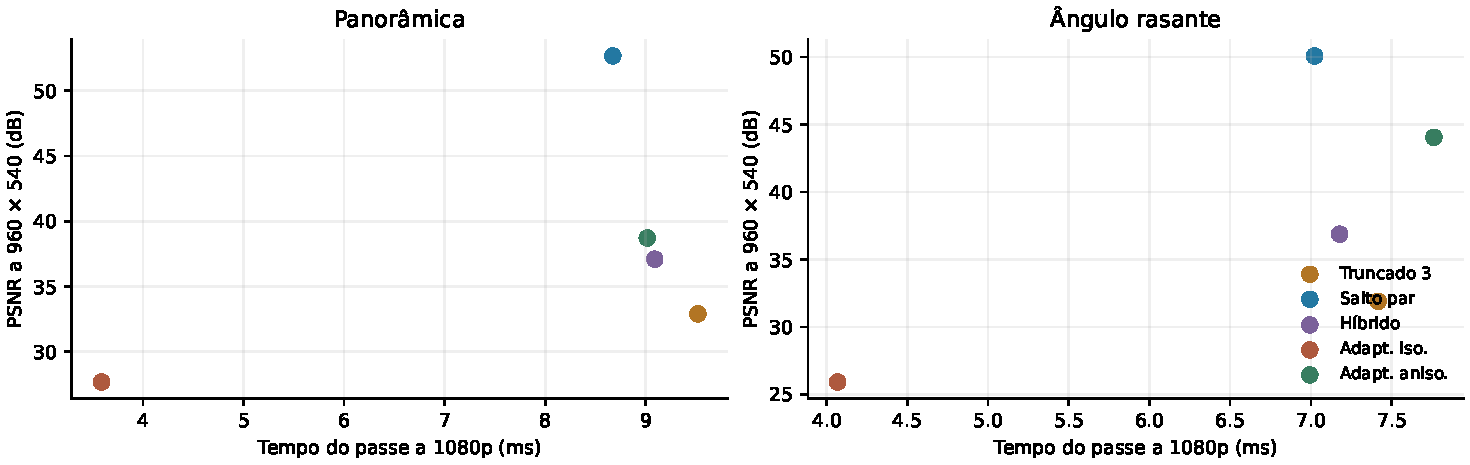
\includegraphics[width=0.97\textwidth]{figures/compromisso.pdf}
\caption{Compromisso observado em PBR 2. O eixo horizontal usa tempos a 1080p; o vertical, PSNR de renderizações separadas a $960\times540$. O completo é omitido por ter PSNR infinito contra si. O gráfico combina indicadores de resoluções distintas e não constitui uma fronteira de Pareto a resolução única.}
\label{fig:tradeoff}
\end{figure*}

\section{Protocolo v2 e validação automatizada}
\label{sec:v2}
\subsection{Resolução comum e rastreabilidade}
As limitações identificadas na avaliação histórica motivaram a implementação de um segundo protocolo. Em v2, cada caso usa a mesma largura e altura no alvo de temporização, na captura RGBA, no cálculo de PSNR/SSIM e na telemetria. O par de imagens para ambas as métricas é o mesmo; a máscara de terreno vem do canal alfa. A etapa Python confere as dimensões reais dos PNGs, recalcula PSNR e verifica sua concordância com o valor obtido no navegador, com tolerâncias absoluta e relativa de $10^{-9}$. O SSIM usa a janela $11\times11$ e exclui centros cujo suporte ultrapasse o terreno ou a imagem, sem recorrer a uma máscara menos restritiva quando não existem janelas válidas.

A leitura de pixels e a codificação das imagens ocorrem antes da temporização. O passe temporizado continua incluindo terreno e céu, enquanto as métricas consideram apenas o terreno. Cada captura é exportada por etapas para evitar acumular múltiplas imagens 4K simultaneamente em memória. Os arquivos registram dimensões, método, referência, estimador de seleção e filtro inicial, e os validadores rejeitam resultados com resoluções incompatíveis ou células ausentes na matriz de métodos.

O registro de consultas foi substituído por um histórico individual com identificadores de sessão, caso, método, rodada e posição na ordem de execução. Cada consulta preserva fase, instante de submissão, disponibilidade, estado de disjunção e, quando válida, duração em nanossegundos e milissegundos. Os estados finais distinguem coleta válida, aquecimento válido, disjunção, expiração e resultado inválido. Uma disjunção invalida todas as consultas pendentes, inclusive aquelas ainda indisponíveis, evitando que uma consulta contaminada seja aceita em uma leitura posterior.

Para cada método, a contagem de consultas solicitadas deve ser igual à soma de válidas e descartadas. Os agregados são recalculados a partir das consultas aceitas; aquecimento não entra nas estatísticas. São exportados média, mediana, quartis, IQR, P95, desvio padrão descritivo e causas de descarte. O protocolo científico exige o timer de GPU, sem substituição silenciosa por um cronômetro de CPU. O runner identifica renderização por software, que é tolerada apenas quando explicitamente habilitada para validação funcional.

O comando de coleta completa foi configurado para cinco sessões, cada uma em um processo e perfil novos de navegador. Por caso, o padrão é de 60 renderizações iniciais, cinco rodadas de aquecimento e 100 rodadas de coleta, com ordem direta/reversa alternada. O resumo mantém as medianas de cada sessão e calcula sua mediana e IQR entre sessões, sem tratar consultas de uma mesma sessão como repetições independentes. Esses valores são escolhas explícitas de protocolo; sua implementação não demonstra, por si só, convergência do aquecimento ou estabilidade estatística.

\subsection{Ablação e controle negativo}
A Equação~\ref{eq:lodseparado} permite uma matriz fatorial $2\times2$: estimador de seleção isotrópico ou anisotrópico, combinado com filtragem inicial por \texttt{textureGrad} ou \texttt{textureLod}. O LOD usado na amostragem dos níveis posteriores permanece anisotrópico e fixo entre as células. Os identificadores \texttt{adap\_iso} e \texttt{adap\_aniso} agora compartilham o filtro inicial \texttt{grad}; as duas células adicionais usam o sufixo \texttt{\_lod}. Por isso, os números antigos de \texttt{adap\_iso} não são intercambiáveis com os de v2, apesar da semelhança do nome.

Além de conferir parâmetros, implementamos um controle negativo sobre imagens realmente renderizadas. Nele, os limiares são elevados para $n=2$ e $f=3$, acima de $\xi\in[0,\,1]$, mantendo todos os fragmentos no regime completo. Com pesos de regime constantes, trocar somente o estimador de seleção deve produzir os mesmos pixels para um filtro fixo. O teste exige identidade contra a referência nas células \texttt{grad}, com PSNR infinito e SSIM unitário, e igualdade dos PNGs entre as duas células \texttt{lod}. O controle passou nos dois enquadramentos de teste. Ele detectaria o acoplamento anterior em que o estimador alterava também os mipmaps amostrados, embora não substitua a análise de todas as condições possíveis.

\subsection{Suíte e resultados funcionais}
A suíte de validação combina casos em Node.js (\texttt{node:test}) e em Python, executados sob \texttt{npm test}. Foram aprovados 25 testes automatizados, um dos quais executa cinco verificações em Python com valores de referência de PSNR/SSIM, máscara e suporte da janela. Os demais verificam a matriz de ablação, as estatísticas, a exclusão de aquecimento, a preservação de consultas, os estados de descarte e a rejeição de relatórios inconsistentes. Testes com contexto de GPU simulado exercitam disjunção antes da disponibilidade e expiração; os testes de integração usam o shader real.

As integrações foram executadas em Chrome headless 136, Windows, WebGL 2 via ANGLE/D3D11, sobre uma NVIDIA GeForce RTX 4050 Laptop GPU, com suporte ao timer de GPU. O ambiente de orquestração usou Node.js 24.11.1 e Python 3.12.14. Os dois testes de \texttt{npm run test:gpu} cobrem duas sessões independentes em $320\times180$ e $640\times360$, seguidas do controle negativo em uma terceira sessão. O teste \texttt{npm run test:gpu:resolutions} acrescenta uma quarta sessão, com panorâmica em 1080p e rasante em 4K. Todas as quatro sessões foram concluídas.

Foram preservados 288 registros de consultas: 216 de coleta válidas e 72 de aquecimento válido, sem descartes nesses casos. Cada sessão cobre 18 combinações de caso/método, incluindo as quatro células adaptativas e cinco comparadores. A configuração curta usa três rodadas de coleta e uma de aquecimento por método, além de seis renderizações iniciais. Ela verifica execução e consistência; não constitui a coleta científica de cinco sessões e 100 rodadas descrita anteriormente.

\begin{table*}[t]
\centering\small\setlength{\tabcolsep}{4pt}
\caption{Validação funcional do protocolo v2 na RTX 4050. PSNR e SSIM usam as mesmas capturas RGBA e dimensões da temporização. Os enquadramentos diferem entre as colunas; esta tabela não mede escalabilidade de resolução. Cada linha tem três consultas de coleta válidas por caso, sem descartes.}
\label{tab:v2quality}
\begin{tabular}{lrrrr}\toprule
 & \multicolumn{2}{c}{1080p, panorâmica} & \multicolumn{2}{c}{4K, rasante}\\
Método & PSNR (dB) & SSIM & PSNR (dB) & SSIM\\\midrule
Linear & 32,65 & 0,963659 & 31,17 & 0,985847\\
Completo 6 & $\infty$ & 1,000000 & $\infty$ & 1,000000\\
Truncado 3 & 32,52 & 0,957478 & 31,76 & 0,985509\\
Salto par & 51,99 & 0,999317 & 50,03 & 0,999633\\
Híbrido & 37,09 & 0,984116 & 36,89 & 0,994978\\
Adaptativo iso./grad & 35,12 & 0,969095 & 40,03 & 0,990984\\
Adaptativo aniso./grad & 42,18 & 0,988397 & 50,77 & 0,998220\\
Adaptativo iso./lod & 28,02 & 0,844573 & 29,52 & 0,927398\\
Adaptativo aniso./lod & 28,90 & 0,858891 & 29,96 & 0,931633\\
\bottomrule\end{tabular}
\end{table*}


A Tabela~\ref{tab:v2quality} apresenta as métricas das capturas coincidentes com as resoluções temporizadas. Com filtro inicial \texttt{grad} mantido constante, o adaptativo anisotrópico obtém 42,18 dB contra 35,12 dB do isotrópico na panorâmica a 1080p, e 50,77 contra 40,03 dB na rasante a 4K. Os SSIMs correspondentes são, respectivamente, 0,988397 contra 0,969095 e 0,998220 contra 0,990984. Esses dois casos fornecem evidência de uma diferença de fidelidade associada à seleção de regimes sob filtragem controlada. Não estabelecem superioridade em materiais ou enquadramentos não avaliados.

As células \texttt{lod} apresentam PSNR menor contra a referência comum \texttt{grad}, evidenciando que a filtragem inicial é um fator distinto e relevante. A comparação não atribui todo esse desvio à política adaptativa, pois a própria referência usa outro filtro. O salto par permanece próximo da referência, com 51,99 dB na panorâmica a 1080p e 50,03 dB na rasante a 4K. A Figura~\ref{fig:v2frames} mostra as capturas com filtragem inicial constante.

\begin{figure*}[t]
\centering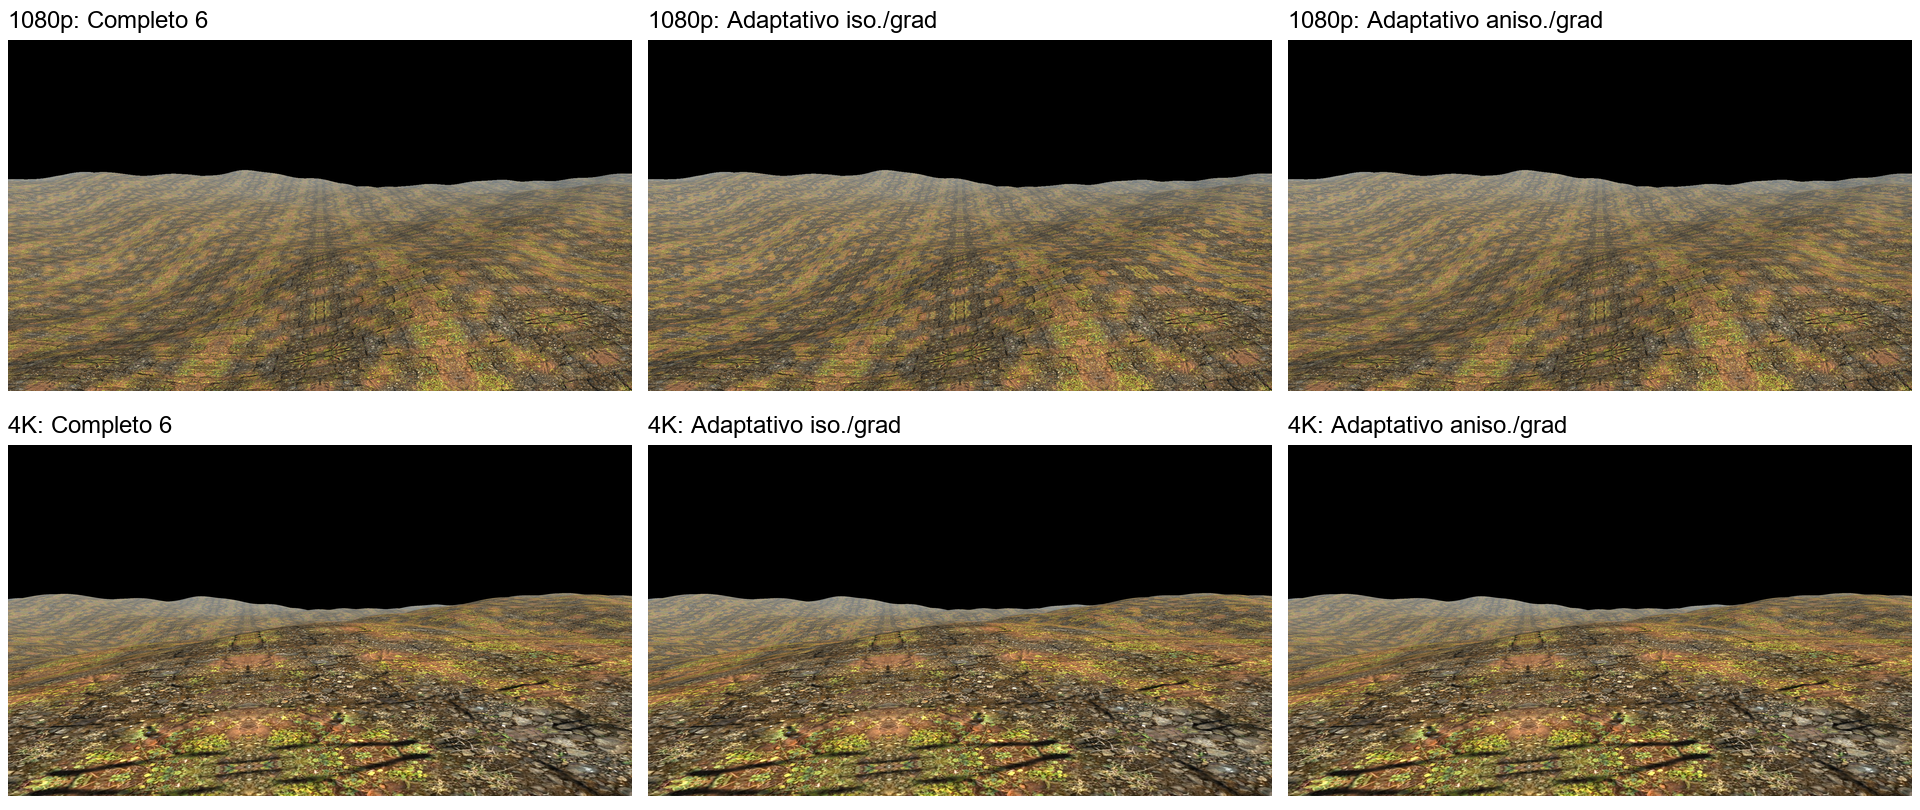
\includegraphics[width=0.97\textwidth]{figures/validacao_v2.png}
\caption{Capturas do protocolo v2 na RTX 4050: completo, adaptativo isotrópico e adaptativo anisotrópico, todos com filtro inicial \texttt{grad}. Linha superior: panorâmica a 1080p; inferior: rasante a 4K. As imagens foram reduzidas apenas para compor a figura; as métricas usam os PNGs originais. O fundo preto corresponde aos pixels fora do terreno excluídos pela máscara alfa.}
\label{fig:v2frames}
\end{figure*}

Os tempos individuais da coleta curta são disponibilizados para auditoria da instrumentação, mas não usados para anunciar novas reduções de desempenho ou comparar a RTX 4050 com a GPU AMD histórica. Além da troca de hardware, o algoritmo de seleção/filtragem e o protocolo mudaram. O ganho principal demonstrado nesta etapa é metodológico: as dimensões coincidem, as consultas podem ser auditadas e o fator de seleção possui um controle de independência em pixels. A coleta completa permanece necessária para concluir sobre estabilidade dos tempos e o novo compromisso custo--qualidade.


\section{Discussão}
\subsection{Resposta às questões de pesquisa}
A primeira hipótese é sustentada no conjunto avaliado: o salto par fica mais próximo da reconstrução de seis bandas que o truncamento 3, sob a mesma contagem lógica. Sua diferença de PSNR na GPU PBR 2 é 19,76 dB na panorâmica e 18,20 dB na rasante. Além disso, o salto apresenta menor tempo médio que o truncamento nessas configurações. Como a contagem de amostras é igual, a diferença de tempo não pode ser explicada apenas pela quantidade de chamadas; a distribuição dos níveis e o caminho de execução também importam.

O resultado do híbrido precisa ser interpretado com cautela. Preservar a primeira banda não compensa automaticamente a ausência do residual 6. Seu PSNR próximo do truncamento até 5 sugere que a diferença de suporte macroscópico domina parte da discrepância. Uma comparação futura deve incluir $\{0,\,1,\,3,\,6\}$ ou $\{0,\,1,\,3,\,5,\,6\}$ para separar esses efeitos, explicitando os respectivos custos. Este estudo não testa essas novas sequências e não presume seu desempenho.

A segunda hipótese foi inicialmente apoiada apenas como comparação de caminhos completos em v1, devido à mudança simultânea de estimador e filtragem. A ablação v2 mantém o filtro e o LOD de amostragem constantes ao comparar os seletores; nos dois casos da Tabela~\ref{tab:v2quality}, o anisotrópico se aproxima mais da referência. O controle negativo acrescenta evidência de que o seletor não altera diretamente a filtragem quando os pesos são fixados. A conclusão permanece limitada aos enquadramentos e ativos examinados; diferenças de tempo entre seletores ainda precisam de coleta completa sob esse protocolo.

\subsection{Quando a adaptação compensa}
A Figura~\ref{fig:tradeoff} mostra que o caminho mais rápido pode ter fidelidade substancialmente menor. O isotrópico é rápido porque, além de selecionar menos reconstrução, usa uma filtragem diferente da referência. O salto par ocupa uma região de alta fidelidade com custo intermediário e dispensa limiares dependentes da cena. O adaptativo anisotrópico oferece uma alternativa quando diferenças maiores são aceitáveis e há cobertura suficiente de regiões distantes.

Na câmera rasante a 1080p, porém, o salto par é simultaneamente mais rápido e mais próximo da referência no PSNR registrado que o adaptativo anisotrópico. Portanto, a política adaptativa não domina o salto fixo. O reuso remove redundâncias de amostragem, mas não elimina a aritmética de reconstruções simultaneamente ativas nem garante ramificações uniformes entre fragmentos. O resultado prático depende do hardware, da resolução e dos limiares.

A diferença entre amostras lógicas e tempo também aparece na mudança de resolução. Na panorâmica PBR 2, o adaptativo anisotrópico passa de aproximadamente 21,42 amostras médias a 1080p para 29,27 a 4K, contra 35 na referência. A redução lógica diminui de 38,8\% para 16,4\%; a redução de tempo cai de 20,8\% para 6,5\%. Esses valores têm relação coerente com a política de LOD, mas não demonstram proporcionalidade entre amostras e banda efetiva de memória.

\subsection{Validade das métricas}
PSNR e SSIM medem proximidade de uma referência específica. Não determinam se a imagem de referência é a preferida por um observador, se o material é fisicamente plausível ou se a mistura preserva todas as estatísticas das fontes. Em especial, SSIM arredondado a 1,0000 pode coexistir com erro finito e overshoot. O uso de quatro casas na tabela não deve ser interpretado como igualdade numérica.

As máscaras também mudam a sensibilidade da avaliação: na rampa ampla, grande parte da imagem já se aproxima da mistura de máscara constante; na máscara orgânica, diferenças se concentram em transições complexas. Métricas globais diluem alterações esparsas. Uma avaliação adicional deve registrar distribuições de erro por região e percentis de erro angular, além de médias. Recortes dirigidos ao erro, como os apresentados, complementam a inspeção, mas não fornecem estimativa de frequência de falhas numa população de materiais.

Como verificação de sensibilidade da região de SSIM, recalculamos os oito pares de quadros preservados das câmeras panorâmica e rasante com erosão $11\times11$, compatível com o suporte da janela. A maior variação absoluta em relação à erosão histórica $9\times9$ foi 0,000528. A ordenação entre salto par, adaptativo anisotrópico, linear e adaptativo isotrópico permaneceu igual nas duas câmeras. Esse teste reduz a preocupação com a escolha de margem nesses quadros, sem resolver as diferenças de resolução ou a ausência de avaliação temporal.

O overshoot bruto da decomposição não equivale a pixels inválidos na imagem entregue, porque existe recorte ou renormalização posterior. Por outro lado, essas correções podem modificar energia e orientação. Um estudo de aparência especular deveria variar a rugosidade e a iluminação de forma independente, observar a distribuição de normais e comparar sequências animadas. Os mapas de rugosidade sintéticos desta implementação não substituem esse protocolo.

\section{Limitações e ameaças à validade}
\subsection{Dados, referência e generalização}
O conjunto é pequeno e compartilha ativos entre casos. Rotação, reutilização de textura e derivação de uma terceira camada introduzem variações controladas, mas não constituem uma amostra ampla de materiais naturais e produzidos. Não avaliamos histogramas preservados como baseline, texturas HDR, mapas com canais físicos independentes, UVs com distorção extrema ou materiais altamente estruturados. As conclusões se restringem às entradas e ao operador de referência escolhidos.

O caminho offline opera sobre os valores RGB codificados lidos das imagens, e não aplica conversão explícita para radiância linear. O WebGL configura saída linear, mas a comparação não estabelece equivalência colorimétrica completa entre a bancada e os ativos de albedo. Uma submissão voltada a fidelidade física deve definir o espaço de cor de cada mapa, linearizar albedo quando apropriado e manter normais, máscaras e rugosidade como dados. Os resultados atuais descrevem a implementação avaliada.

Os seis níveis da referência são um parâmetro experimental. Uma decomposição menos profunda pode ser artisticamente preferível; assim, a baixa similaridade de um truncamento ao nível 6 não significa necessariamente pior aparência em qualquer uso. A própria escolha do residual define quanto as cores médias são compartilhadas. Nossa primeira hipótese é sobre fidelidade a esse alvo, não sobre uma ordenação universal de operadores.

\subsection{Desempenho e instrumentação}
Os ganhos de tempo históricos vêm de uma única GPU AMD e de uma sessão registrada em v1. Não há série de consultas individuais preservada nem contagem por caso após descarte nessa etapa; a previsão de 25 rodadas não prova o número efetivamente válido. Em v2, o registro individual e a contagem explícita resolvem essa lacuna de instrumentação para novas execuções, mas não recuperam as consultas antigas. A validação na RTX 4050 é uma segunda configuração de hardware, sob outro protocolo e com coleta curta; não constitui reprodução independente dos ganhos históricos. Não fazemos teste de significância, bootstrap ou comparação de desempenho entre os dois dispositivos.

As consultas envolvem o passe de cena, incluindo céu e trabalho geométrico. A preparação de máscaras é excluída, e as máscaras são estáticas durante a coleta. Portanto, os resultados não caracterizam um sistema de máscaras animadas que regenere mipmaps a cada quadro nem o tempo completo de uma aplicação interativa. A taxa de quadros exibida em um HUD não foi usada como substituto do tempo de GPU.

A telemetria conta operações lógicas declaradas pelo shader. Não há perfil de cache, contadores de transações ou medição de utilização de TMUs; a redução teórica não é uma redução medida de banda. Em v1, a grade menor de telemetria e seu fator de derivadas apenas aproximam o alvo temporizado. Em v2, a telemetria é renderizada nas mesmas dimensões do caso, eliminando essa aproximação espacial, sem transformar o contador lógico em contador físico de hardware.

\subsection{Resolução, anisotropia e comportamento temporal}
A separação de resoluções entre qualidade e tempo limita os gráficos históricos de compromisso: a política adaptativa reage à pegada por pixel. Os PSNRs repetidos em v1 não estabelecem fidelidade a 4K. As novas capturas e métricas de v2 usam as dimensões correspondentes da temporização, inclusive 4K, resolvendo essa incompatibilidade para os novos casos. Contudo, panorâmica e rasante não formam um par de câmera idêntica entre resoluções na validação curta; a Tabela~\ref{tab:v2quality} não é um estudo de escalabilidade. A coleta completa, com enquadramentos correspondentes e sessões adicionais, é necessária para caracterizar o compromisso de desempenho do algoritmo corrigido.

Os mapas de normais usam resolução diferente do albedo, enquanto o indicador comum de seleção é parametrizado por resolução de referência de 1024. A normalização do LOD é uma decisão prática do material composto, não uma adaptação independente de cada mapa. Isso limita a interpretação de igualdade de alcance físico dos níveis entre canais e sugere separar o cálculo de pegada por resolução de mapa em testes futuros.

Por fim, as imagens são estáticas. A função \texttt{smoothstep} garante pesos contínuos no parâmetro de seleção, mas não fornece garantia temporal após minificação, amostragem discreta e mudanças de visibilidade. Não medimos erro entre quadros, cintilação sob movimento de câmera, atualização dinâmica da máscara ou taxas de troca de regime. A afirmação de eliminação completa de popping seria, portanto, mais forte que a evidência disponível.

\section{Conclusão}
Avaliamos a seleção de níveis na mesclagem Laplaciana por três perspectivas complementares: reconstrução offline, simulação de terreno e tempo registrado em GPU. O salto par $\{0,\,2,\,4,\,6\}$ preserva o residual da referência e oferece o compromisso mais consistente entre as configurações de alta fidelidade avaliadas. No albedo 2D, supera o truncamento 3 de mesmo orçamento em 21,77 dB; no PBR 2 das quatro câmeras a 1080p, reduz o tempo médio do passe em 14,9--25,3\%, com PSNR de 50,09--54,33 dB medido separadamente a $960\times540$.

A seleção adaptativa histórica evidencia a importância da anisotropia e a dependência do enquadramento, mas não melhora simultaneamente tempo e fidelidade em todos os casos. O protocolo v2 separa o estimador de seleção da filtragem e do LOD de amostragem, unifica as resoluções e preserva cada consulta. Seus 25 testes rápidos e três testes de integração foram aprovados, incluindo controle negativo em pixels e capturas reais em 1080p/4K. Nos novos casos com filtro inicial constante, o adaptativo anisotrópico alcança 42,18 dB na panorâmica a 1080p e 50,77 dB na rasante a 4K, contra 35,12 e 40,03 dB do isotrópico. A coleta curta valida funcionamento e fornece evidência de fidelidade, sem estabelecer novos ganhos de tempo.

Como continuação, é necessário executar a coleta completa já implementada, com cinco sessões e 100 rodadas por método, avaliar estabilidade do aquecimento e ampliar materiais, dispositivos e condições de câmera. A avaliação temporal de câmera e máscara animadas e a normalização explícita de espaços de cor permitirão testar outros limites. A identidade telescópica e a formulação do erro organizam a interpretação, enquanto testes e consultas auditáveis tornam explícitas as condições empíricas. Os resultados apoiam o salto par no cenário estudado e fornecem uma base controlada para avaliar o custo do método adaptativo corrigido.

\section*{Disponibilidade e uso de ferramentas}
O código e os dados-base correspondem à revisão \texttt{10293a4} do repositório \url{https://github.com/ViniciusMBotelho/laplacian-texture-blending}, branch \texttt{checkpoint-2-trabalho}; o protocolo v2, os testes e esta versão do manuscrito estão organizados na branch \texttt{benchmark-validacao}. O pacote contém fontes LaTeX, figuras, tabela gerada e quatro registros JSON de validação, com consultas individuais e manifesto SHA-256. Os PNGs brutos são gerados pelos comandos de teste e identificados por hashes no manifesto, mas não integram o pacote leve versionado. A documentação inclui comandos de reprodução e distingue coleta curta de coleta científica completa. A documentação anterior registra assistência do Google Gemini; esta consolidação utilizou ChatGPT/Codex para auditoria, redação técnica, conferência bibliográfica, instrumentação e testes automatizados. As medições históricas são separadas das novas validações. A aprovação científica, autoral e editorial final cabe aos autores e ao orientador.

\balance
\bibliography{referencias}
\end{document}
